\documentclass[
  bibliography=totoc,     % Literatur im Inhaltsverzeichnis
  captions=tableheading,  % Tabellenüberschriften
  titlepage=firstiscover, % Titelseite ist Deckblatt
]{scrartcl}

% Paket float verbessern
\usepackage{scrhack}

% Warnung, falls nochmal kompiliert werden muss
\usepackage[aux]{rerunfilecheck}

% unverzichtbare Mathe-Befehle
\usepackage{amsmath}
% viele Mathe-Symbole
\usepackage{amssymb}
% Erweiterungen für amsmath
\usepackage{mathtools}

% Fonteinstellungen
\usepackage{fontspec}
% Latin Modern Fonts werden automatisch geladen
% Alternativ zum Beispiel:
%\setromanfont{Libertinus Serif}
%\setsansfont{Libertinus Sans}
%\setmonofont{Libertinus Mono}

% Wenn man andere Schriftarten gesetzt hat,
% sollte man das Seiten-Layout neu berechnen lassen
\recalctypearea{}

% deutsche Spracheinstellungen
\usepackage[main=ngerman]{babel}


\usepackage[
  math-style=ISO,    % ┐
  bold-style=ISO,    % │
  sans-style=italic, % │ ISO-Standard folgen
  nabla=upright,     % │
  partial=upright,   % ┘
  warnings-off={           % ┐
    mathtools-colon,       % │ unnötige Warnungen ausschalten
    mathtools-overbracket, % │
  },                       % ┘
]{unicode-math}

% traditionelle Fonts für Mathematik
\setmathfont{Latin Modern Math}
% Alternativ zum Beispiel:
%\setmathfont{Libertinus Math}

\setmathfont{XITS Math}[range={scr, bfscr}]
\setmathfont{XITS Math}[range={cal, bfcal}, StylisticSet=1]

% Zahlen und Einheiten
\usepackage[
  locale=DE,                   % deutsche Einstellungen
  separate-uncertainty=true,   % immer Fehler mit \pm
  per-mode=symbol-or-fraction, % / in inline math, fraction in display math
]{siunitx}

% chemische Formeln
\usepackage[
  version=4,
  math-greek=default, % ┐ mit unicode-math zusammenarbeiten
  text-greek=default, % ┘
]{mhchem}

% richtige Anführungszeichen
\usepackage[autostyle]{csquotes}

% schöne Brüche im Text
\usepackage{xfrac}

% Standardplatzierung für Floats einstellen
\usepackage{float}
\floatplacement{figure}{htbp}
\floatplacement{table}{htbp}

% Floats innerhalb einer Section halten
\usepackage[
  section, % Floats innerhalb der Section halten
  below,   % unterhalb der Section aber auf der selben Seite ist ok
]{placeins}

% Seite drehen für breite Tabellen: landscape Umgebung
\usepackage{pdflscape}

% Captions schöner machen.
\usepackage[
  labelfont=bf,        % Tabelle x: Abbildung y: ist jetzt fett
  font=small,          % Schrift etwas kleiner als Dokument
  width=0.9\textwidth, % maximale Breite einer Caption schmaler
]{caption}
% subfigure, subtable, subref
\usepackage{subcaption}


% Grafiken können eingebunden werden
\usepackage{graphicx}
% größere Variation von Dateinamen möglich
%\usepackage{grffile}

% schöne Tabellen
\usepackage{booktabs}

% Verbesserungen am Schriftbild
\usepackage{microtype}
\setlength{\parindent}{0pt}

% Literaturverzeichnis
\usepackage[
  backend=biber,
]{biblatex}
% Quellendatenbank
\addbibresource{lit.bib}
\addbibresource{programme.bib}

% Hyperlinks im Dokument
\usepackage[
  german,
  unicode,        % Unicode in PDF-Attributen erlauben
  pdfusetitle,    % Titel, Autoren und Datum als PDF-Attribute
  pdfcreator={},  % ┐ PDF-Attribute säubern
  pdfproducer={}, % ┘
]{hyperref}
% erweiterte Bookmarks im PDF
\usepackage{bookmark}

% Trennung von Wörtern mit Strichen
\usepackage[shortcuts]{extdash}

% Import PDFs
\usepackage{pdfpages}


\usepackage{graphicx}






\title{Compton-Effekt\\
\small{Versuch 608}
}
\author{%
  Marcel Kebekus\\%
  \href{mailto:marcel.kebekus@tu-dortmund.de}{marcel.kebekus@tu-dortmund.de}%
}
\date{%
  Abgabe: 5.05.2020 
}
\publishers{TU Dortmund – Fakultät Physik}
\makeatletter         
\def\@maketitle{
\raggedright
\includegraphics[width=\textwidth]{bilder/lo_TU-Do 2008/logo_rgb_jpg}\\[8ex]
\begin{center}
{\Huge \bfseries \sffamily \@title }\\[4ex] 
{\Large  \@author}\\[4ex] 
\@date\\[8ex]
\publishers\\
\end{center}}
\makeatother


\begin{document}


\maketitle
\thispagestyle{empty}
\tableofcontents
\newpage
\newpage
\section*{Zielsetzung}
Aufnehmen und analysieren von dem Emissionsspektrum einer CU-
Röntgenröhre und verschiedener Absorbtionsspektren.
\section{Theorie}
\subsection{Erzeugung Röntgenstrahlung}
Innerhalb einer evakuierten Röhre werden Elektronen aus einer Glühkathode
auf eine Anode hin beschleunigt.\\ 
Die Energie der Strahlung kann mithilfe der Bragg-Reflexion ermittelt werden.
Durch Beugung an einem dreidimsensionalen Gitter (LiF-Kristall) mit der Gitterkonstante $d$ 
entsteht eine konstruktive Interferenz bei einem Braggwinkel $\Theta$. Durch die Bragg-Bedingung
\begin{equation}
    2 d \sin(\Theta)=n\lambda,
    \label{eqn:bragg}
\end{equation}
ergibt sich die Wellenlänge $\lambda$. n ist dabei die Beugungsordunung.
\begin{figure}
    \centering
    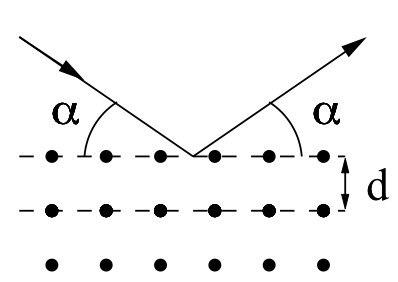
\includegraphics[width=0.3\textwidth]{plots/bragg.jpg}
    \caption{Darstellung der Bragg-Reflexion an einem Gitter mit der
    Gitterkonstante $d$ und dem Bragg-Winkel $\alpha$.\cite[3]{anleitung}}
\end{figure}
\\Die Röntgenstrahlung ist auf zwei Effekt zurückzuführen.


\subsubsection*{Charakteristisches Spektrum}
Beim Auftreffen der Elektronen auf das Anodenmaterial wird dieses ionsisiert, sodass
ein gebundenes Elektron von einer höheren Schale auf eine niedrigere Schale fallen kann und dabei
Energie in Form von Röntgenquanten imitiert. Die abgestrahlte Energie entspricht dann der Differenz
der Energieniveaus.
\begin{equation}
    h\cdot v=E_m-E_n
\end{equation}
Das charakteristische Spektrum ist vom Anodenmaterial abhängig und zeichnet sich im
Röntgenspektrum durch schwarfe Linien aus.
Für ein Elektron in einem Mehrelektronenatom ergibt sich die Energie durch
\begin{equation}
    E_n=-R_{\infty}\cdot z_{\text{eff}}^2 \cdot \frac{1}{n^2},
\end{equation}
wobei die Rydbergenergie $R_{\infty}=13.6$eV und die effektive Kernladung 
$z_{eff}=z-\sigma$ mit der Abschirmkonstante $\sigma$ ist. Dabei wird berücksichtigt,
dass die Hüllenelektronen die Coulomb Anziehung auf das äußere Elektron abschirmen.
\begin{figure}
    \centering
    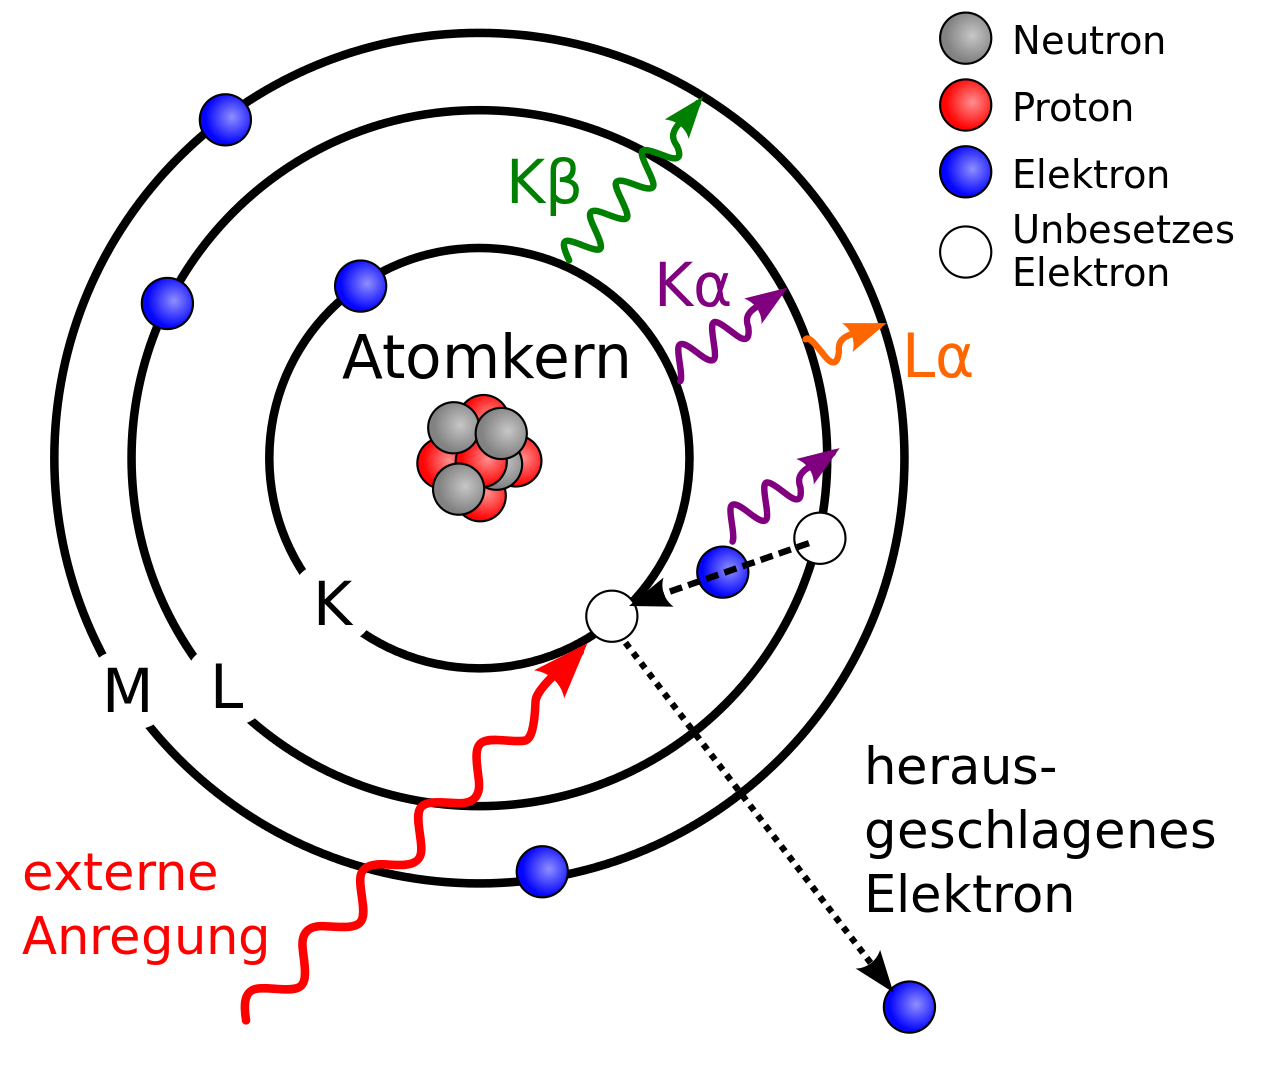
\includegraphics[width=0.4\textwidth]{plots/chS.png}
    \caption{Darstellung des Prozesses der Röntenemission durch die
    Ionisation des Atoms. Das (Röntgen)Photon wirkt als exteren Anregung, welches
    ein Elektron aus der inneren Schale schlägt. Ein anderes Elektron aus einer
    höheren Schale rutscht nach und gibt Energie in Form von Strahlung ab.\cite{wiki}}
\end{figure}

\subsubsection*{Bremsstrahlung}
Durch Abbremsen der freien Elektronen in einem Elektrischen Feld 
wird Energie durch Röntgenquanten frei. Die Energie entspricht dabei
dem Energieverlust der Abbremsung. Bei vollständiger Abbremsung ergibt
sich die Wellenlänge
\begin{equation}
    \lambda_{min}=\frac{h \cdot c}{e_0U}.
    \label{eqn:minW}
\end{equation}
Da hierbei verschieden hohe kinetische Energien abgegeben werden können,
äußert siche die Bremsstrahlung im Spektrum durch einen Kontinuierlichen
Verlauf.
\subsection{Halbwertsbreite (Full Width at Half Maximum)}
Die Breite bie halber Höhe (kurz: FWHM) beschreibt "die Differenz zwischen 
den beiden Argumentwerten, für die die Funktionswerte auf die 
Hälfte des Maximums abgesunken sind."\cite{wiki2}
\begin{figure}
    \centering
    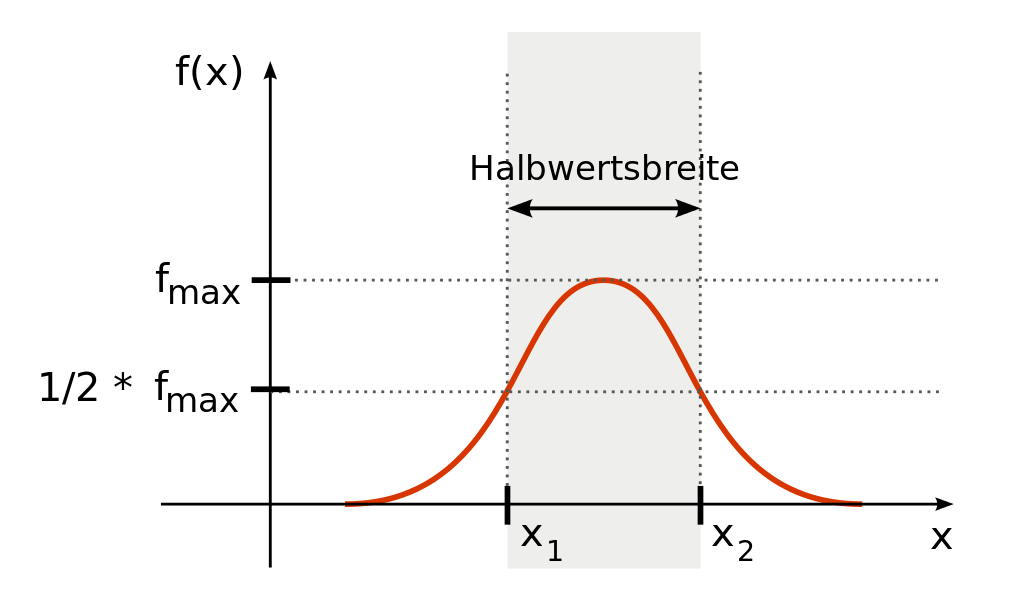
\includegraphics[width=0.4\textwidth]{plots/Halbwertsbreite.png}
    \caption{}
\end{figure}
\subsection{Absorbtion}
Treffen Röntgenstrahlen auf ein Material, so nimmt dieses die Strahlung zum Teil
auf (Absorbtion). Diese ist zum Teil vom Material, derer Dicke $d$ und der Energie 
der Strahlung abhängig.
\begin{equation}
    \frac{I(d)}{I_0}=e^{-\mu d}=:\tau
\end{equation}
Dabei ist $\mu$ der Absorbtionskoeffizient.\\
Dieser ist abhängig von der Energie der Strahlung und nimmt bei zunehmender
Strahlungsenergie ab. $\mu$ steigt sprunghaft an, wenn die Strahlungsenergie
gleich groß der Bindungsenergie eines Elektrons aus der nächsten inneren Schale ist.
Man spricht von einer Absorbtinskante.
Für die K-Kante (n=1) ergibt sich nach der Sommerfledschen Feinstrukturformel
die Abschirmkonstante
\begin{equation}
    \sigma_K=Z-\sqrt{\frac{E_K}{R_{\infty}}-\frac{\alpha^2Z^4}{4}}
    \label{eqn:sigmaZ}
\end{equation}
Da die Elektronen in einer Schale nicht alle die selbe potenzielle Energie
besitzen spalten sich die Hauptkanten auf in eng an einanerliegene Linien (Feinstrukturen),
diese werden im folgenden allerdings nicht weiter aufgelöst.\\
So folgt für eine Abschätzung der Abschirmkonstanten $\sigma$ für Kupfer
mit $n=1$,$m=2$ und $l=3$,
\begin{align}
    \sigma_1 &= Z-\sqrt{\frac{E_{K,abs}}{R}},\\
    \sigma_2 &= Z-\sqrt{4\cdot (Z-\sigma_1)^2-\frac{4E_{K\alpha}}{R}}, \\
    \sigma_3 &= Z-\sqrt{9\cdot(Z-\sigma_1)^2-\frac{9E_{K\beta}}{R}} .
    \label{eqn:sigma}
\end{align}

Bei Strahlungsenergien unterhalb von $1$MeV treten erstmal Compton- und Photoeffekt ein.
\subsection{Mosley'sch Gesetz}
Nach 
\begin{equation}
    E_K=Rh(z-\sigma)^2
    \label{eqn:mos}
\end{equation}
ist die Energie der $K_{\alpha}$-Strahung proprtional zu $z^2$ bei $n=1$.




\newpage
\section{Durchführung}
\subsection{Messschaltung}
Die Ladungen $Q$ die sich am Anodendraht sammeln fließen über einen
Wiederstand $R$ ab und werden über einen Spannungsimpuls über einen Kondensator $C$
ausgekoppelt, über einen Verstärker vergrößert und somit vom Zählgerät regristriert.
\begin{figure}
    \centering
    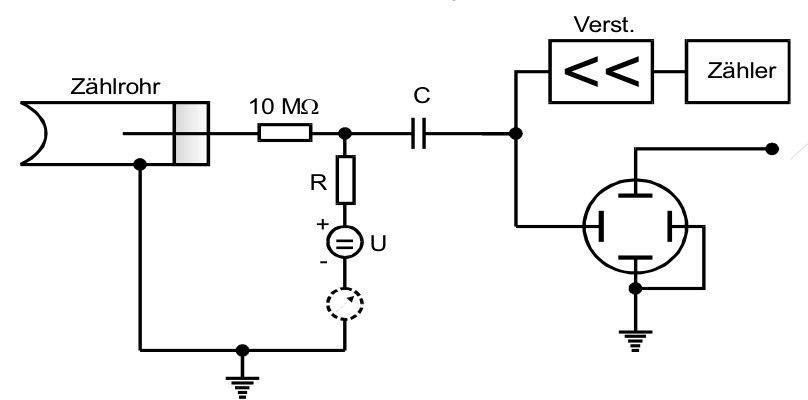
\includegraphics[width=0.7\textwidth]{input/messapperatur.jpg}
    \caption{\cite[226]{anleitung}}
\end{figure}

\subsection{Aufnahme der Charakteristik}
Gemessen wird die Zählrate einer $\beta$-Quelle in Abhängigkeit der Betriebsspannung $U$.
$U \leq 700\si{V}$ sollte dabei eingehalten werden, um das Zählrohr durch
einen zuhohen Intensitätsstrom nicht zu zerstören. Zudem übersteigt die Impulsrate nicht $100\;/\;\si{s}$
damit die Totzeit-Korrektur vermieden werden kann.\\
Gemessen wir hierfür die Anzahl der Zerfälle pro Zeitintervall in Schritten von $\Delta U=10\si{V}$.
\subsection{Bestimmung der Totzeit}
Für die Bestimmung der Totzeit können zwei Methoden genutzt werden.
\subsubsection*{Oszilloskop}
Durch Ablesen der ersten beiden Peaks am Oszilloskop, welche die Spannungsimpulse graphisch visulaisiert,
kann die Totzeit direkt bestimmt werden
\subsubsection*{Zwei-Quellen-Methode}
Mit einer zusätzlichen $^{204}Tl$-Quelle die näher an das Geiger-Müller Zählrohr gerückt ist,
lässt sich über Gl. \ref{eqn:2Quellen} mit den gemessenen Zählraten die Totzeit $T$ berechnen.
\subsection{Bestimmung des Zählrohrstroms}
Mithilfe Gl. \ref{eqn:strom} kann aus dem mittleren Zählstrom $I$
die freigesetzten Ladungen pro eingefallendem Teilchen berechnet werden. 
\label{sec:Durchfuehrung}

\newpage
\newpage
\section{Auswertung}
Die charakteristischen Strahlung/Peaks im Röntgenspektrum sind abbhängig vom 
verwendeten Annodenmaterial Kupfer. Die Linien befinden sich bei \cite{literatur}
\begin{align*}
    K_{\alpha}=8,038\si{keV},\\
    K_{\beta}=8,905\si{keV},
\end{align*}
und somit liegen sie bei den Wellenlängen (Gl. \ref{eqn:energie})
\begin{align*}
    \lambda_{\alpha} =& \frac{hc}{E_{K_{\alpha}}}\approx 1,6\cdot 10^{-10}\si{m},\\
    \lambda_{\beta}  =& \frac{hc}{E_{K_{\beta}}}\approx 1,4 \cdot 10^{-10}\si{m} .
\end{align*}
Dieser Wellenlänge wird nach Gl. \ref{eqn:bragg} und Gl. \ref{eqn:energie} der Braggwinkel $\alpha$ 
mit der Gitterkonstante $d=201,4\cdot 10^{-12}$ von
\begin{align*}
    \alpha_{K_{\alpha}}=&sin^{-1}\left(\frac{hc}{2d \cdot E_{K_{\alpha}}}\cdot\right)\approx 23°,\\
    \alpha_{K_{\beta}}=&sin^{-1}\left(\frac{hc}{2d \cdot E_{K_{\beta}}}\cdot\right)\approx 21°,
\end{align*}
zugeordnet.

\begin{figure}[H]
    \centering
    \includegraphics[width=0.65\textwidth]{plots/welll_int.pdf}
    \caption{Die Impulsrate $I_0$ gegen den Braggwinkel $\alpha$ und die 
    Röntgenwellenlänge $\lambda$ aufgetragen. Es zeigten sie die Peaks der 
    charakteristischen Strahlung, sowie der Berg der Bremsstrahlung, der ab einem 
    Winkel $\alpha=8°$ bis zum ersten Peak verläuft. Die Beschleunigungsspannung 
    beträgt $35$kV.}
    \label{fig:braggw}
\end{figure}

\begin{figure}[H]
    \centering
    \includegraphics[width=0.65\textwidth]{plots/E_int.pdf}
    \caption{Das Energiespektrum der Röntgenstrahlung. Es zeigen sich
    die charakteristischen Röntgenstrahlen bei $K_{\alpha}=8,05$keV und 
    $K_{\beta}=8,92$keV}
    \label{fig:energie}
\end{figure}


Man entnimmt den Messdaten und aus Abb. \ref{fig:energie} und Abb. \ref{fig:braggw} 
folgende charakteristische Strahlungswerte
\begin{align*}
    K_{\alpha}=&8,05keV &\alpha_{K\alpha}=&22,5°& \lambda_{K\alpha}=&154,14\si{pm}\\ 
    K_{\beta}=&8,92keV &\alpha_{K\beta}=&20,2° &\lambda_{K\beta}=&139,09\si{pm}\\
\end{align*}



\subsection{Wellenabhängigkeit der Tansmission}
Um eine Aussage über die Abhängigkeit der Transmission von der Wellenlänge
zu machen, müssen die gemessenen Impulsraten $N_0$ und $N_1$ über Gl. \ref{eqn:totzeit}
mit der Totzeit $\tau=90\mu$s korrigiert werden. Die Transmission ergibt sich dann aus dem Quotienten
von $I_0$ und $I_1$
\begin{equation}
    T_0=\frac{I_1}{I_0}.
    \label{eqn:trans}
\end{equation}
Trägt man nun die aus den Braggwinkel mithilfe der Bragg'schen Reflexion
berechneten Wellenlänge $\lambda$ gegen die Transmission $T$ auf, so folgt
nach linearer Regression über die Geradengleichung
\begin{equation*}
    T=m\cdot \lambda + n,
\end{equation*}
mit der Steigung $m$ und dem y-Achsenabschnitt $n$
\begin{align*}
    m=&(-15.20\pm0.23)\cdot 10^{-9}\si{W\per\m^3},\\ 
    n=&(1.231\pm0.014)\cdot 10^{-12}\si{W\per\m^2},
\end{align*}
die Abhängigkeit $T(\lambda).$
\begin{figure}[H]
    \centering
    \includegraphics[width=0.65\textwidth]{plots/trans.pdf}
    \caption{Gezeigt ist die prozentuale Transmission $T$, die der Wellenlänge $\lambda$
    gegenübergestellt ist. Die lineare Regression zeigt den Zusammenhang $T(\lambda)$.
    Verwendet wurde ein Aluminium Absorber.}
\end{figure}
\label{sub:trans}


\subsection{Die Compton-Wellenlänge}
Bei gleichem Streuwinkel wurden nun die Intensität für compton-gestreute Photonen
$I_{gestreut}$ mit Al-Absorber,nicht gestreute Photonen $I_{ungestreut}$, sowie 
die Intensität $I_0$ ohne Absorber gemessen.
Nun kann über die Transmission und den bereitgestellen Zusammenhang (vgl. Abschnitt \ref{sub:trans})
$T(\lambda)$ die Wellenlänge der Compton-Strahlung bestimmt werden.
Die Poisson verteilten Röntgen-Quanten mit der Messunsicherheit\\
\begin{align*}
    \Delta N= \sqrt{N},
\end{align*}
ergeben für die Impulse
\begin{align*}
    I_0=(2730\pm50)\si{Impulse},\\
    I_{gestreut}=(1024\pm32)\si{Impulse},\\
    I_{ungestreut}=(1180\pm34)\si{Impulse}.
\end{align*}
Es ergibt sich für die Transmission T
\begin{align*}
    T_{ungestreut}=\frac{I_{ungestreut}}{I_{0}}=(0.432\pm0.015)\%,\\
    T_{gestreut}=\frac{I_{gestreut}}{I_{0}}=(0.375\pm0.014)\%.
\end{align*}
Aus dem Zusammenhang $T(\lambda)$ folgt dafür
\begin{align*}
    \lambda_{ungestreut}=(52.6\pm1.6)\si{pm},\\
    \lambda_{gestreut}=(56.3\pm1.5)\si{pm}.
\end{align*}
Es folgt somit für die Compton-Wellenlänge $\lambda_C$ nach \ref{eqn:compton} mit
einem Streuwinke von $90$°
\begin{equation*}
    \lambda_C=\lambda_{gestreut}-\lambda_{ungestreut}=(3.8\pm1.1)\si{pm}.
\end{equation*}
\label{sec:Auswertung}

\newpage
\section{Diskussion}

\newpage
\section{Anhang}
\begin{figure}
    \centering
    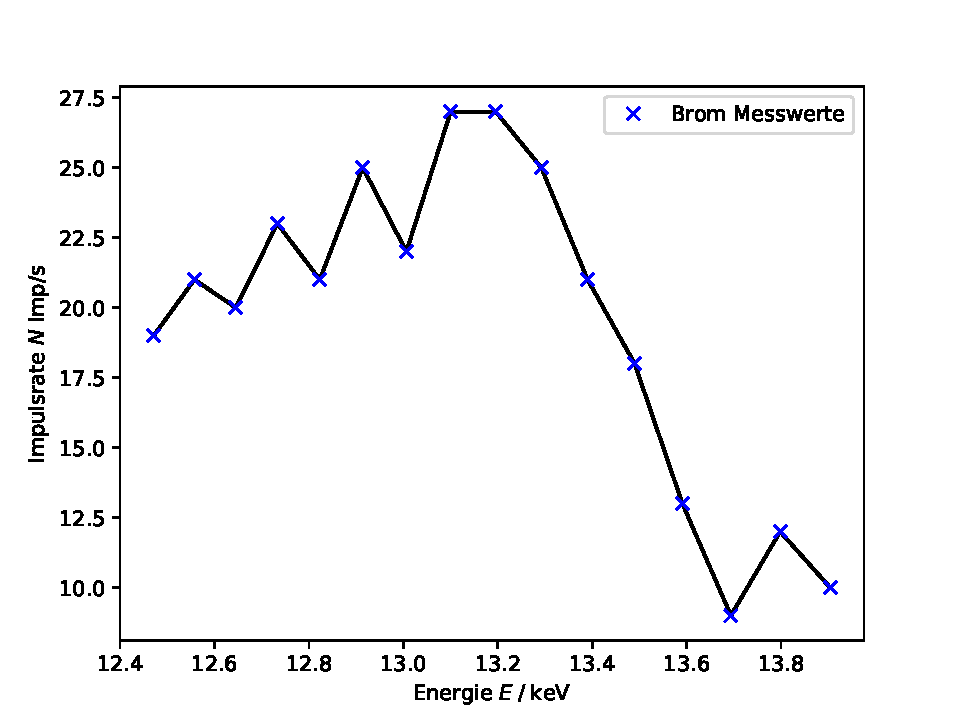
\includegraphics[width=0.7\textwidth]{plots/Brom.pdf}
    \caption{}
\end{figure}
\begin{figure}
    \centering
    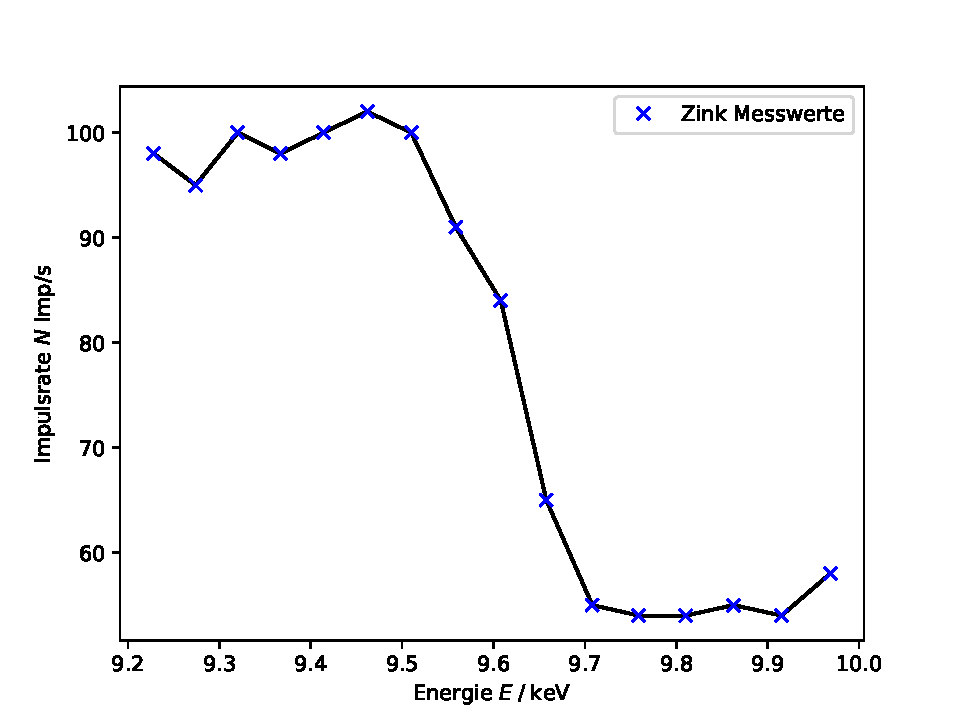
\includegraphics[width=0.7\textwidth]{plots/Zink.pdf}
    \caption{}
\end{figure}
\begin{figure}
    \centering
    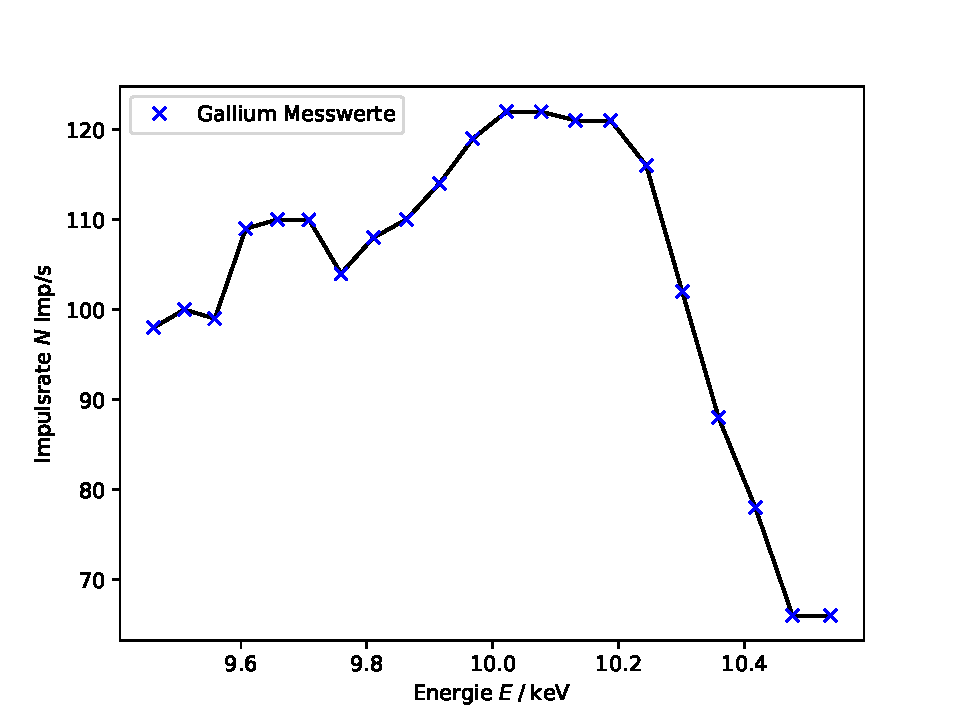
\includegraphics[width=0.7\textwidth]{plots/Gallium.pdf}
    \caption{}
\end{figure}
\begin{figure}
    \centering
    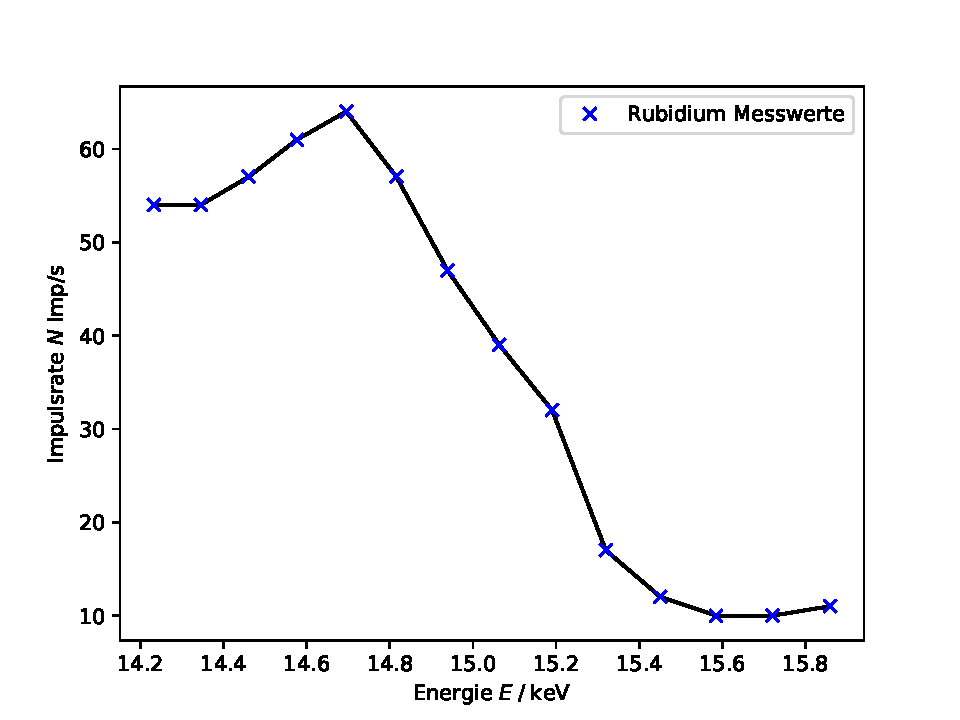
\includegraphics[width=0.7\textwidth]{plots/Rubidium.pdf}
    \caption{}
\end{figure}
\begin{figure}
    \centering
    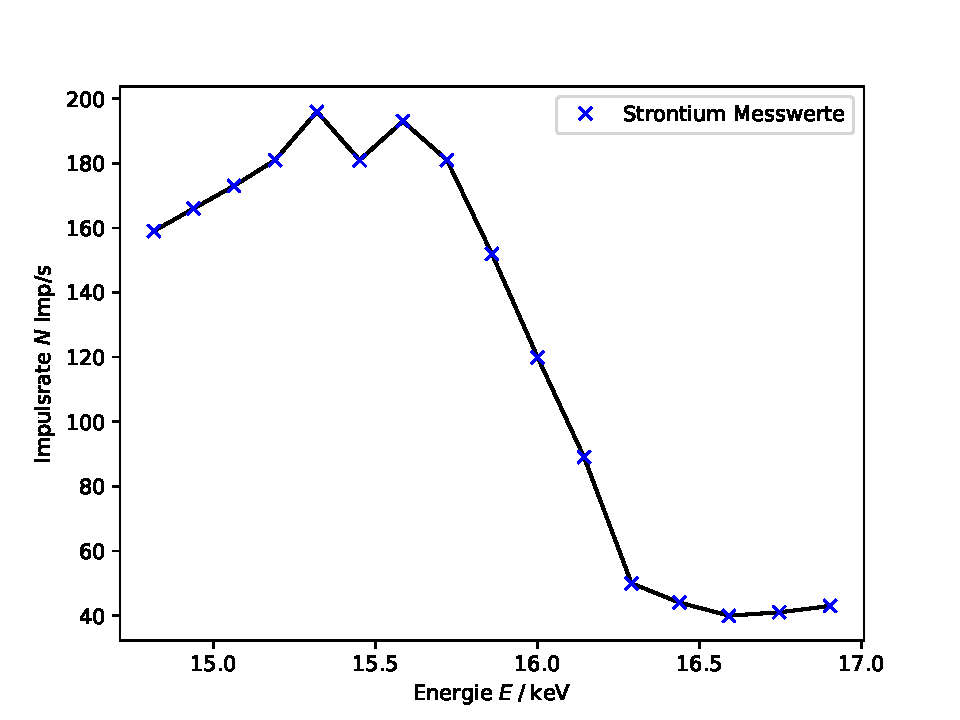
\includegraphics[width=0.7\textwidth]{plots/Strontium.pdf}
    \caption{}
\end{figure}
\begin{figure}
    \centering
    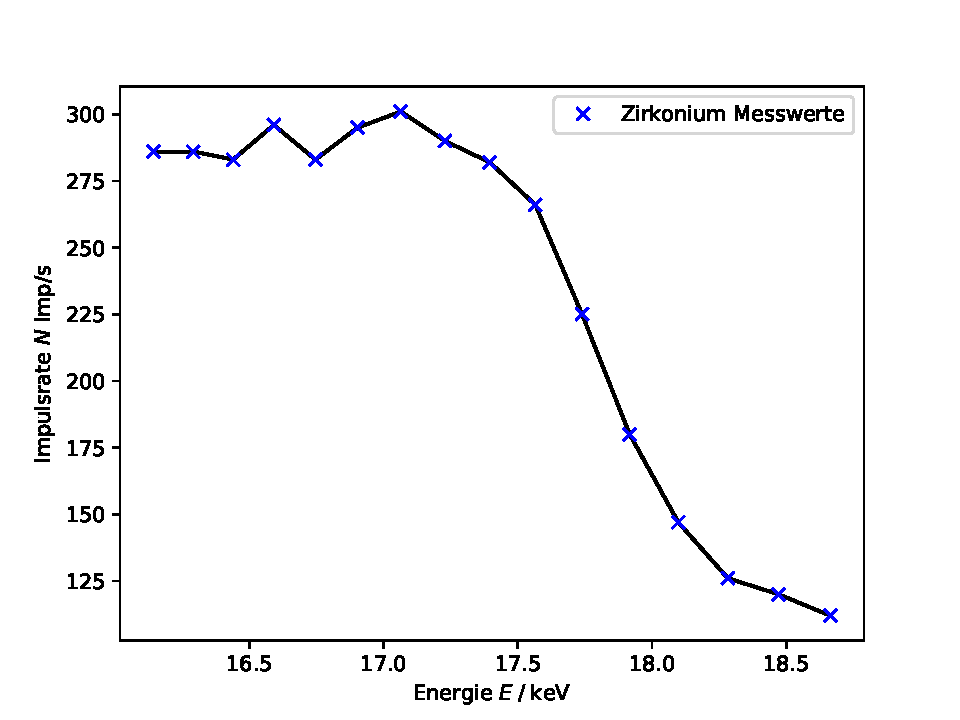
\includegraphics[width=0.7\textwidth]{plots/Zirkonium.pdf}
    \caption{}
\end{figure}
\label{sec:anhang}


\newpage
\nocite{*}
\printbibliography


\end{document}
